\documentclass{beamer}
\usepackage{pgfpages}
\usepackage[english]{babel}
\usepackage[T1]{fontenc}
\usepackage[latin1]{inputenc}
\usepackage{color}
\usepackage{float}

\usepackage{pgfplots}
\usepackage{pgfplotstable}
\usepackage{tikz}
\pgfplotsset{scale=0.6, compat=1.7}


\mode<presentation>
{
    \usetheme{Warsaw}
    \useoutertheme[subsection=false]{miniframes}
    \usefonttheme[onlylarge]{structuresmallcapsserif}
    \setbeamercovered{transparent}
}
\pagestyle{empty}
\thispagestyle{empty}


\begin{document}

%%%%%%%% HISTORY %%%%%%%%%%%%%%%%%%%
\begin{frame}
\frametitle[Gravitational Constant]{Motivation}

   \begin{itemize}
   \item  Henry Cavendish Made an Experiment to determine the density of the Earth.
   \item  This was later picked up by others and used to figure out G.
   \item The literature value for G is ${6.67\times 10^{-11}}m^{3}kg^{-1}s^{2}$
   \end{itemize}
\end{frame}

%%%%%%%% Methods %%%%%%%%%%%%%%%%%%%

\begin{frame}
\frametitle[Gravitational Constant]{Two Methods}

   \begin{itemize}
   \item  End Deflection
   \item  Acceleration
   \end{itemize}
   
   \centering
   \begin{figure}
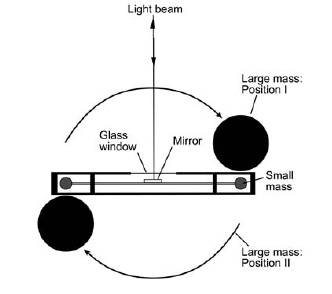
\includegraphics[width=4cm, height=4cm]{images/cav2.png}
\label{fig:cab}
\end{figure}
\end{frame}

\begin{frame}
\frametitle[Gravitational Constant]{Set Up}

   \begin{itemize}
   \item  End Deflection
   \item  Acceleration
   \end{itemize}
   
   \centering
   \begin{figure}
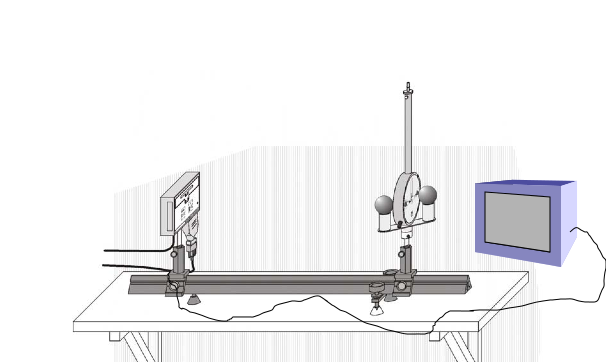
\includegraphics[width=7cm, height=5cm]{images/edit.png}
\label{fig:cab}
\end{figure}
\end{frame}



\begin{frame}
\frametitle[Gravitational Constant]{Set Up}
   
   \centering
   \begin{figure}
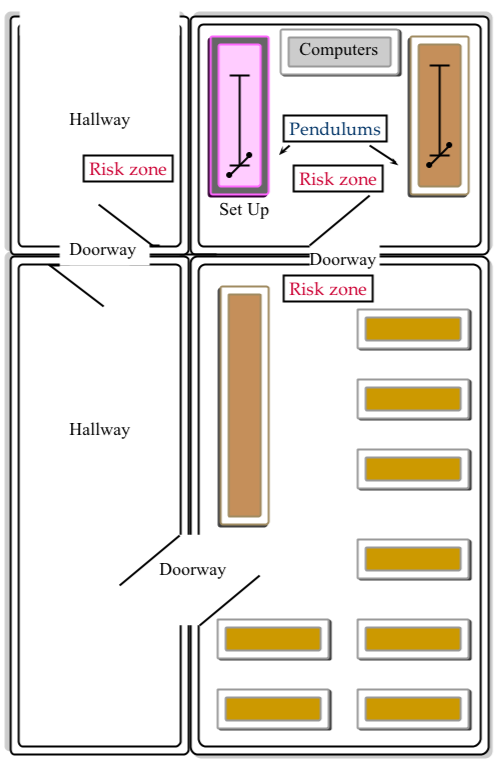
\includegraphics[width=5.5cm, height=5cm]{images/map.png}
\label{fig:cab}
\end{figure}
\end{frame}


\begin{frame}
\frametitle[Gravitational Constant]{End Deflection}

 
   Difference between equilibrium positions
$$G=\frac{\pi^{2}{d}{b}^{2}}{T^{2}m_{2} }cos{\beta}$$

\end{frame}


\begin{frame}
\frametitle[Gravitational Constant]{Acceleration}
   \begin{itemize}
   \item  First minute: Not Enough data points
   \item  Not Very Reproducible 
   \item $a_{o}$ is the slope of linear graph
   \end{itemize}

$$G=\frac{b^2 a_{o} d}{ 2 m^{2}} cos\beta$$

\end{frame}



\begin{frame}
\frametitle[Gravitational Constant]{Main Result}

\begin{figure}[H]
\centering
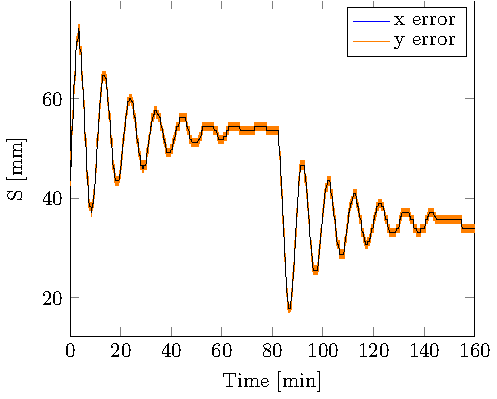
\includegraphics[width=7cm, height=4cm]{graphs/mainresult}
\caption{Main result. The x error bars are too small to see. The y error bars are in orange. $6.56(2))\times{10}^{-11} m^{3}kg^{-1}s^{2}$}
\label{fig:mainresult}
\end{figure}
\end{frame}

\begin{frame}
\frametitle[Gravitational Constant]{Acceleration}

\begin{figure}[H]
\centering
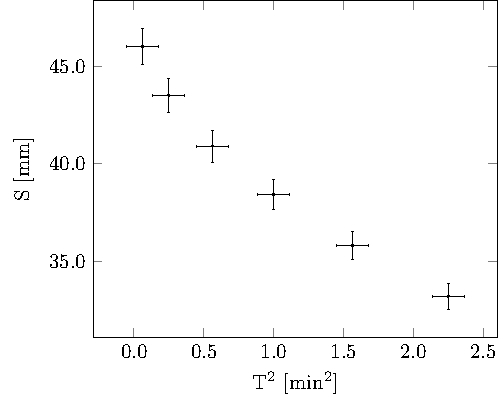
\includegraphics[width=6cm, height=4cm]{images/linear}
\caption{Acceleration from the second curve sloping downwards. The first six points were recorded up to 1.5 minutes. This yielded a result of $6.68(2)\times{10}^{-11} m^{3}kg^{-1}s^{2}$}
\label{fig:mainresult}
\end{figure}
\end{frame}

\begin{frame}
\frametitle[Gravitational Constant]{Systematic Errors}
  \framesubtitle{Need to resolve forces}
  $$m_{1}a=\frac{G m_{1}m_{2}}{b^{2}}$$

\begin{figure}[H]
\centering
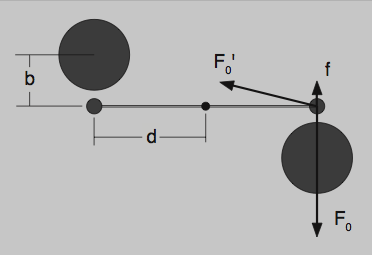
\includegraphics[width=6cm, height=4cm]{images/Forces}
\caption{A Schematic of the forces involved in the calculation}
\label{fig:forces}
\end{figure}
\end{frame}


\begin{frame}
\frametitle[Gravitational Constant]{Errors}
\centering
\begin{itemize}
\item The Acceleration was analysed using a java program
\item end deflection was analysed using CASSY Lab
\end{itemize}

\end{frame}

\begin{frame}
\frametitle[Gravitational Constant]{Errors}
\centering
$$\sqrt{\left(\frac{\partial^{2}{G}}{\partial{}{a}^{2}}\Delta{a}\right)^{2}
+\left(\frac{\partial^{2}{G}}{\partial{b}^{2}}\Delta{b}\right)^{2}}$$

For b, d, $m_{1rf}$ and $\Delta{S}$ and the error on L cancelled out $\frac{L_{o}}{L}$.
\end{frame}


\begin{frame}
\frametitle[Gravitational Constant]{Questions?}


\end{frame}
\end{document}